% Vilnius University beamer template
% Created in 2024 by Joana Katina

\documentclass[12pt]{beamer}
% You can use \documentclass[11pt,aspectratio=169]{beamer} 
% to adjust the aspect ratio to 16:9.
\renewcommand{\figurename}{}
\renewcommand{\tablename}{}
\renewcommand\thefigure{\arabic{figure} figure.}
\renewcommand\thetable{\arabic{table} table.}

\usepackage{graphicx}
\usepackage{listings}
\usepackage[
	backend=biber,
	style=numeric,
	sorting=ynt
]{biblatex}
\usepackage{algorithm,algorithmic}
\usepackage{caption}
\captionsetup{justification=centering}
\captionsetup[table]{font=scriptsize,justification=centering}


\usepackage{biblatex}
\usepackage{hyperref}
\usepackage{subfig}

% ---- added for the paradox slides ----
\usepackage{amsmath,amssymb}
\usepackage{booktabs}
\usepackage{multirow}
\usepackage{array}
\usepackage{tikz}
\usepackage{pgfplots}
\pgfplotsset{compat=1.17}
\usetikzlibrary{arrows.meta}
% Green block for the game examples
\definecolor{gamegreen}{RGB}{46,125,50}
\newenvironment{gameblock}[1]{%
  \setbeamercolor{block title}{bg=gamegreen,fg=white}%
  \setbeamercolor{block body}{bg=gamegreen!8}%
  \begin{block}{#1}}{\end{block}}
\newcommand{\X}{\mathcal{X}}

\addbibresource{references.bib}

\usetheme{Madrid}

\title[Paradoxes of Choices under Uncertainty]{Paradoxes of Choices under Uncertainty}
\subtitle[]{Microeconomic analysis}
\author[Ber\v{z}inskas, Skuodas, \v{Z}itkevi\v{c}ius]{Gedas Ber\v{z}inskas, Adrijus Skuodas, Jok\={u}bas \v{Z}itkevi\v{c}ius}
\date{}

%% Supervisor
\addtobeamertemplate{author}{}{Supervisor: Assoc. Dmitrij Celov\par}

\setbeamertemplate{navigation symbols}{}
\titlegraphic{
\includegraphics[width=2cm]{resources/MIF.png}}

\usepackage{VUMIF}
\usepackage[T1]{fontenc}

\begin{document}

% Title slide
\begin{frame}
  \titlepage
\end{frame}

% Outline
\begin{frame}{Outline}
  \tableofcontents
\end{frame}

\section{Expected utility: the benchmark}

\begin{frame}{Choices under uncertainty}

A \textbf{lottery} specifies possible outcomes and their probabilities:
\[
L=\{(x_1,p_1),\ldots,(x_n,p_n)\}, \quad
p_i\geq 0,\quad \sum_{i=1}^n p_i=1,\quad
x_i\in\mathcal{X}.
\]

\vspace{-0.15cm}
\begin{itemize}
    \item Outcomes may be monetary prizes; probabilities describe
    their chances.
    \item A decision-maker has preferences over lotteries, written
    $L\succeq M$ if $L$ is weakly preferred to $M$.
    \item The question: can these preferences be represented by
    a consistent rule?
\end{itemize}

\vspace{0.1cm}
\begin{block}{Expected value is not enough}
Two lotteries can have the same expected monetary payoff but be
ranked differently because the decision-maker responds to risk.
\end{block}

\end{frame}

\begin{frame}{Example: a lottery in Minecraft}
\small
\begin{gameblock}{Mining a diamond ore with a \emph{Fortune III} pickaxe}
The game draws the number of diamonds you get:
\[
L_{\text{mine}}=\Big\{(1,\tfrac25),\ (2,\tfrac15),\ (3,\tfrac15),\ (4,\tfrac15)\Big\},
\qquad \mathbb{E}[L_{\text{mine}}]=\tfrac{2+2+3+4}{5}=2.2 .
\]
A villager offers instead: \textbf{2 diamonds for sure} for the unmined ore.
\end{gameblock}
\begin{itemize}
  \item Risk-neutral player: $2.2>2$ $\Rightarrow$ mine it.
  \item A careful hardcore player who needs exactly 2 diamonds may take the sure 2.
  \item Both are reasonable: we need a rule that ranks \emph{lotteries}, not just their averages.
\end{itemize}
\end{frame}

\begin{frame}{Expected utility}
\scriptsize

Assign each outcome $x$ a utility $u(x)$, where
$u:\mathcal{X}\rightarrow\mathbb{R}$.
The expected utility of a lottery is
\[
EU(L)=\sum_{i=1}^n p_i u(x_i).
\]

The model predicts that
\[
L\succeq M
\quad\Longleftrightarrow\quad
EU(L)\geq EU(M).
\]

This representation is justified by the
\textbf{von Neumann--Morgenstern expected utility theorem}.
Preferences must be:
\begin{itemize}
    \item \textbf{complete and transitive},
    \item \textbf{continuous}, and
    \item satisfy \textbf{independence}.
\end{itemize}

\vspace{0.05cm}
\begin{alertblock}{Independence: the key axiom}
If $L\succeq M$, then for any lottery $N$ and
$0<\alpha<1$,
\[
\alpha L+(1-\alpha)N
\succeq
\alpha M+(1-\alpha)N.
\]
Adding the same lottery component to both options should not
reverse their ranking.
\end{alertblock}

\end{frame}

\begin{frame}{Independence axiom}
\small

Suppose $L\succeq M$. Independence requires
\[
\alpha L+(1-\alpha)N
\succeq
\alpha M+(1-\alpha)N,
\qquad \alpha>0.
\]

Under expected utility, the difference between the two
mixtures is
\[
\begin{aligned}
&EU\bigl(\alpha L+(1-\alpha)N\bigr)\\
&\quad-EU\bigl(\alpha M+(1-\alpha)N\bigr)\\
&=\alpha EU(L)+(1-\alpha)EU(N)\\
&\quad-\alpha EU(M)-(1-\alpha)EU(N)\\
&=\alpha\bigl[EU(L)-EU(M)\bigr].
\end{aligned}
\]

Since $\alpha>0$, the sign of the difference is unchanged.

\begin{block}{Prediction}
A common lottery component cannot reverse the ranking
between two lotteries.
\end{block}

\end{frame}

\begin{frame}{Independence in plain words: a Skyrim dungeon}
\small
\begin{gameblock}{Two chests behind a door}
W.p.\ $1-\alpha$ a draugr ambush ends the run (lottery $N$). W.p.\ $\alpha$ you reach the treasure room and pick chest $L$ (\textbf{500 gold for sure}) or chest $M$ (0 or 1200 gold, 50--50).
\end{gameblock}
\begin{itemize}
  \item The ambush does not depend on the chest you pick.
  \item If you prefer $L$ in the room, you should prefer ``door, then $L$'' to ``door, then $M$'': \ $\alpha L+(1-\alpha)N\succeq\alpha M+(1-\alpha)N$.
\end{itemize}
\begin{alertblock}{The paradoxes}
In experiments people \textbf{systematically break} this rule.
\end{alertblock}
\end{frame}

\section{St.\ Petersburg paradox}

\begin{frame}{St.\ Petersburg paradox: the villager's coin}
\small
\begin{gameblock}{A villager offers a game}
A coin is flipped until the first tails. If tails first appears on flip $k$, you win $2^k$ emeralds. How many emeralds would you pay to play?
\end{gameblock}
\[
\Pr(k)=2^{-k},\qquad
\mathbb{E}[\text{prize}]=\sum_{k=1}^{\infty}2^{-k}\cdot 2^{k}=1+1+1+\dots=\infty .
\]
\begin{itemize}
  \item A risk-neutral player should pay \emph{any} price.
  \item In practice almost nobody pays more than $\approx$ 5--20 emeralds.
\end{itemize}
\begin{block}{Paradox}
Expected \emph{value} gives an absurd answer (Bernoulli, 1738).
\end{block}
\end{frame}

\begin{frame}{Bernoulli's resolution: concave utility}
\small
With wealth $w$ and $u(x)=\ln x$, the maximum price $p$ solves
\vspace{-4pt}
\[
\sum_{k=1}^{\infty}2^{-k}\ln\!\big(w+2^{k}-p\big)=\ln w .
\]
\begin{columns}[T]
\begin{column}{0.48\textwidth}
\centering
\small
\begin{tabular}{rr}
\toprule
Wealth $w$ & Price $p$ \\
\midrule
10 & 4.97\\
100 & 7.79\\
1\,000 & 10.95\\
1\,000\,000 & 20.87\\
\bottomrule
\end{tabular}

\smallskip
{\footnotesize (numerical solution, see Appendix)}
\end{column}
\begin{column}{0.5\textwidth}
\begin{itemize}
  \item Each extra emerald is worth less: $u''<0$.
  \item If the villager owns only $2^{20}\approx10^6$ emeralds, the expected value is just $21$.
\end{itemize}
\end{column}
\end{columns}
\begin{block}{Takeaway}
This paradox \emph{created} EU. But prizes $e^{2^k}$ break log utility again $\Rightarrow$ $u$ must be bounded.
\end{block}
\end{frame}

\section{Allais paradox}

\begin{frame}{Allais paradox: a rare drop in OSRS (vote!)}
\footnotesize
\begin{gameblock}{Old School RuneScape: you got a rare drop. How do you cash it in?}
\textbf{Question 1.} Which do you take?
\begin{itemize}
  \item $A$: sell on the Grand Exchange: \textbf{2\,400k gp for sure}.
  \item $B$: walk it through the Wilderness to a buyer: 2\,500k gp w.p.\ 0.33, 2\,400k w.p.\ 0.66, a player killer takes it w.p.\ 0.01.
\end{itemize}
\pause
\textbf{Question 2.} Two deep-Wilderness trips. Which do you take?
\begin{itemize}
  \item $C$: 2\,500k gp w.p.\ 0.33, nothing w.p.\ 0.67.
  \item $D$: 2\,400k gp w.p.\ 0.34, nothing w.p.\ 0.66.
\end{itemize}
\end{gameblock}
\pause
\begin{block}{Typical answers (Kahneman \& Tversky, 1979)}
82\% choose $A$ and 83\% choose $C$.
\end{block}
\end{frame}

\begin{frame}{Why $A\succ B$ and $C\succ D$ is inconsistent}
\small
Amounts in thousands of gp; normalize $u(0)=0$. Expected utility gives:
\begin{align*}
A\succ B &\iff u(2400) > 0.33\,u(2500)+0.66\,u(2400)\\
         &\iff 0.34\,u(2400) > 0.33\,u(2500),\\[4pt]
C\succ D &\iff 0.33\,u(2500) > 0.34\,u(2400).
\end{align*}
\[
0.34\,u(2400)>0.33\,u(2500)>0.34\,u(2400)\qquad \bot
\]
\begin{block}{Common consequence}
$C,D$ are $A,B$ with the common part ``2\,400 w.p.\ 0.66'' replaced by ``nothing w.p.\ 0.66''. Independence says this cannot matter; people react because $A$ is \textbf{certain}.
\end{block}
\end{frame}

\begin{frame}{The probability triangle (Marschak--Machina)}
\small
\begin{columns}[c]
\begin{column}{0.52\textwidth}
\centering
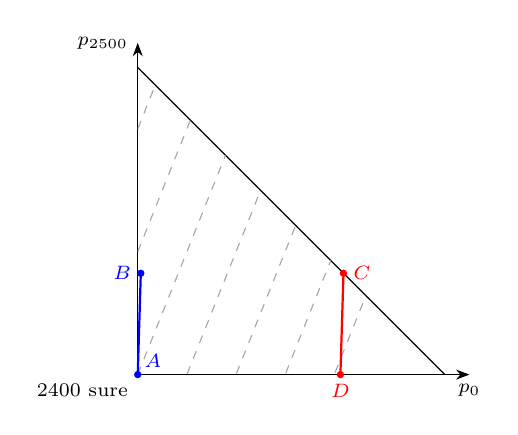
\begin{tikzpicture}[scale=3.9,>=Stealth]
  \draw[->] (0,0) -- (1.08,0) node[below] {\scriptsize $p_{0}$};
  \draw[->] (0,0) -- (0,1.08) node[left] {\scriptsize $p_{2500}$};
  \draw (1,0) -- (0,1);
  \node[below left] at (0,0) {\scriptsize 2400 sure};
  % EU indifference lines: parallel straight lines (illustrative slope)
  \begin{scope}
    \clip (0,0) -- (1,0) -- (0,1) -- cycle;
    \foreach \c in {-1.6,-1.2,-0.8,-0.4,0.0,0.4,0.8}{
      \draw[gray!70,dashed] (0,\c) -- (1,{\c+2.5});
    }
  \end{scope}
  \fill[blue] (0,0) circle (0.012) node[above right=-1pt] {\scriptsize $A$};
  \fill[blue] (0.01,0.33) circle (0.012) node[left] {\scriptsize $B$};
  \fill[red] (0.67,0.33) circle (0.012) node[right] {\scriptsize $C$};
  \fill[red] (0.66,0) circle (0.012) node[below] {\scriptsize $D$};
  \draw[blue,thick] (0,0) -- (0.01,0.33);
  \draw[red,thick] (0.66,0) -- (0.67,0.33);
\end{tikzpicture}
\end{column}
\begin{column}{0.46\textwidth}
\begin{itemize}
\small
  \item Points = lotteries over $\{0,2400,2500\}$.
  \item EU indifference curves: \textbf{parallel lines} (dashed).
  \item $AB \parallel DC$, so EU ranks both pairs alike: $A\succ B \Leftrightarrow D\succ C$.
  \item $A$ and $C$ together need curves that \textbf{fan out}.
\end{itemize}
\end{column}
\end{columns}
\end{frame}

\begin{frame}{Paradoxical pattern of choice}
\scriptsize

Consider four lotteries $L_1,L_2,L_3,L_4 \in \mathcal{L}$ over outcomes $x_1,x_2,x_3 \in \chi$.

Each lottery is represented by a probability distribution:
\[
L_j=\{(x_i,p_{ij})\}_{i=1}^3,
\qquad
\sum_{i=1}^3p_{ij}=1.
\]

Under expected utility, these preferences require
\[
\sum_{i=1}^3p_{i1}u(x_i)>
\sum_{i=1}^3p_{i2}u(x_i),
\]

\[
\sum_{i=1}^3p_{i4}u(x_i)>
\sum_{i=1}^3p_{i3}u(x_i).
\]

\begin{block}{Question}
Can a single utility function satisfy both inequalities
while respecting independence?
\end{block}

\end{frame}

\begin{frame}{Independence and inconsistent preferences}
\small

Without loss of generality, suppose the observed preferences satisfy
\[
L_1\succ L_2,\qquad L_4\succ L_3.
\]

For some \(\alpha\in(0,1)\), let
\[
L_3=\alpha L_1+(1-\alpha)N,\qquad
L_4=\alpha L_2+(1-\alpha)N.
\]

By the independence axiom, \(L_1\succ L_2\) implies \(L_3\succ L_4\). This contradicts the observed preference \(L_4\succ L_3\).

\begin{alertblock}{Conclusion}
The observed reversal violates independence: adding the same lottery component in the same proportions cannot reverse the preference ranking.
\end{alertblock}

\end{frame}

\begin{frame}{Generalized Allais paradox}
\small

Let $x_H>x_M>x_0$, $p,q\in(0,1)$, and define
\[
\begin{aligned}
\mathcal{P}_A&=\delta_{x_M},&
\mathcal{P}_B&=p\delta_{x_H}+(1-p)\delta_{x_0},\\
\mathcal{P}_C&=q\delta_{x_M}+(1-q)\delta_{x_0},&
\mathcal{P}_D&=pq\delta_{x_H}+(1-pq)\delta_{x_0}.
\end{aligned}
\]

Suppose
\[
\mathcal{P}_A\succ\mathcal{P}_B,
\qquad
\mathcal{P}_D\succ\mathcal{P}_C.
\]

Expected utility, with $u(x_0)=0$, implies
\[
\begin{aligned}
u(x_M)&>p\,u(x_H),\\
pq\,u(x_H)&>q\,u(x_M)
\;\Longrightarrow\;
p\,u(x_H)>u(x_M).
\end{aligned}
\]

\[
\boxed{u(x_M)>p\,u(x_H)>u(x_M)}
\qquad\bot
\]

\begin{alertblock}{}
$\text{Violation of independence} \;\Longrightarrow\;
\text{no expected-utility representation.}$
\end{alertblock}
\end{frame}

\begin{frame}{Common ratio effect: a Minecraft expedition}
\small
\begin{gameblock}{Two plans for getting diamonds}
\small
$P_A$: villager trade, \textbf{30 diamonds for sure}.\\
$P_B$: deep cave, \textbf{40 diamonds} w.p.\ 0.8 (a creeper w.p.\ 0.2).\\[3pt]
Same plans, but you first need to find a stronghold (w.p.\ $q=0.25$):\\
$P_C$: 30 w.p.\ 0.25 \qquad $P_D$: 40 w.p.\ $0.25\times0.8=0.20$.
\end{gameblock}
\begin{itemize}
  \item $x_H=40$, $x_M=30$, $x_0=0$, $p=0.8$, $q=0.25$.
  \item Typical: $P_A\succ P_B$ (``sure thing!'') but $P_D\succ P_C$ (``20\% vs 25\%, go for 40'').
\end{itemize}
\begin{block}{}
Scaling all winning chances by $q$ should not change the choice — but it does.
\end{block}
\end{frame}

\section{Ellsberg paradox}

\begin{frame}{Ellsberg paradox: the Khajiit's sack of gems}
\small
\begin{gameblock}{A merchant's sack holds 90 gems}
30 \textbf{rubies}; 60 \textbf{emeralds} or \textbf{sapphires} in an \emph{unknown} mix. Draw one blindly; win 100 gold if your bet is right.
\end{gameblock}
\begin{center}
\begin{tabular}{lccc}
\toprule
Bet & Ruby (30) & Emerald (?) & Sapphire (?)\\
\midrule
I & 100 & 0 & 0\\
II & 0 & 100 & 0\\
\midrule
III & 100 & 0 & 100\\
IV & 0 & 100 & 100\\
\bottomrule
\end{tabular}
\end{center}
\pause
\begin{block}{Typical choice}
I $\succ$ II (``I know it is 1/3'') \ and \ IV $\succ$ III (``I know it is 2/3'').
\end{block}
\end{frame}

\begin{frame}{Why no beliefs can explain it}
\small
Let $\pi_R=\tfrac13$, $\pi_E$, $\pi_S$ be the player's subjective probabilities, $\pi_E+\pi_S=\tfrac23$.
\begin{align*}
\text{I}\succ\text{II} &\iff \pi_R\,u(100) > \pi_E\,u(100) \iff \pi_R>\pi_E,\\
\text{IV}\succ\text{III} &\iff (\pi_E+\pi_S)\,u(100) > (\pi_R+\pi_S)\,u(100) \iff \pi_E>\pi_R .
\end{align*}
\begin{itemize}
  \item Contradiction for \emph{every} belief and \emph{every} $u$.
  \item ``Sapphire'' is a common consequence $\Rightarrow$ Savage's \textbf{sure-thing principle} fails.
\end{itemize}
\begin{block}{Risk vs.\ ambiguity}
Allais: known odds, non-linear attitude to \emph{risk}.\\
Ellsberg: unknown odds, people dislike \textbf{ambiguity}.
\end{block}
\end{frame}

\section{Framing and loss aversion}

\begin{frame}{Framing: Whiterun under dragon attack}
\footnotesize
\begin{gameblock}{A dragon will kill 600 citizens unless the Jarl acts}
\small\textbf{Frame 1 (lives saved):}
\begin{itemize}
  \item Plan A: 200 people will be saved. \hfill [72\%]
  \item Plan B: 1/3 chance 600 saved, 2/3 chance nobody saved. \hfill [28\%]
\end{itemize}
\textbf{Frame 2 (deaths):}
\begin{itemize}
  \item Plan C: 400 people will die. \hfill [22\%]
  \item Plan D: 1/3 chance nobody dies, 2/3 chance 600 die. \hfill [78\%]
\end{itemize}
\end{gameblock}
\begin{block}{Paradox (Tversky \& Kahneman, 1981; Lecture 5)}
A $\equiv$ C and B $\equiv$ D. Only the \emph{words} changed, yet the majority switches: risk-averse for gains, risk-seeking for losses.
\end{block}
\end{frame}

\begin{frame}{Loss aversion and small bets: hardcore mode}
\small
\begin{gameblock}{A 50--50 coin bet in a hardcore world}
Lose 1\,000 emeralds or win 1\,050 emeralds. Do you accept?
\end{gameblock}
\begin{itemize}
  \item Most say \textbf{no}, although the expected value is $+25$.
  \item \textbf{Rabin (2000):} rejecting it at \emph{every} wealth level forces EU to reject a 50--50 bet: lose 20\,000 or win \emph{any} amount. Absurd.
\end{itemize}
\begin{block}{Explanation: losses hurt more than gains please}
With $\lambda\approx2.25$: $0.5\cdot1050-0.5\cdot2.25\cdot1000=-600<0$ $\Rightarrow$ reject.\\
Losing your inventory hurts more than finding the same loot.
\end{block}
\end{frame}

\section{Explaining the paradoxes}

\begin{frame}{Prospect theory (Kahneman \& Tversky)}
\footnotesize
\vspace{-6pt}
{\scriptsize
\[
V(L)=\sum_i w(p_i)\,v(x_i),\quad
v(x)=\begin{cases}x^{\alpha}, & x\ge0\\ -\lambda(-x)^{\beta}, & x<0\end{cases},\quad
w(p)=\frac{p^{\gamma}}{\big(p^{\gamma}+(1-p)^{\gamma}\big)^{1/\gamma}}
\]}
\vspace{-4pt}
{\footnotesize $x$ = gain/loss vs.\ a \textbf{reference point}; $\alpha=\beta=0.88$, $\lambda=2.25$, $\gamma=0.61$.}
\begin{columns}[T]
\begin{column}{0.5\textwidth}
\centering
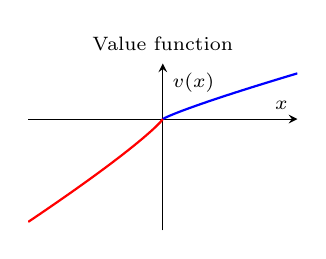
\begin{tikzpicture}
\begin{axis}[width=5.0cm,height=3.7cm,axis lines=middle,xmin=-100,xmax=100,ymin=-140,ymax=70,
  xtick=\empty,ytick=\empty,xlabel={\scriptsize $x$},ylabel={\scriptsize $v(x)$},
  title={\scriptsize Value function},every axis title/.style={at={(0.5,1.02)},anchor=south}]
\addplot[domain=0:100,samples=60,thick,blue] {x^0.88};
\addplot[domain=-100:0,samples=60,thick,red] {-2.25*(-x)^0.88};
\end{axis}
\end{tikzpicture}

{\scriptsize concave for gains, convex and steeper for losses}
\end{column}
\begin{column}{0.5\textwidth}
\centering
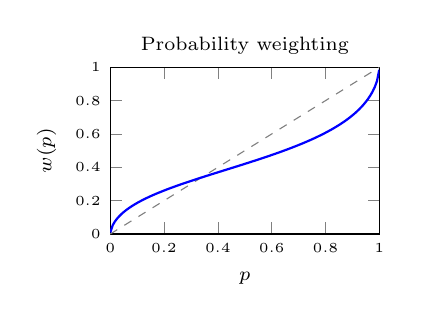
\begin{tikzpicture}
\begin{axis}[width=5.0cm,height=3.7cm,xmin=0,xmax=1,ymin=0,ymax=1,
  xlabel={\scriptsize $p$},ylabel={\scriptsize $w(p)$},tick label style={font=\tiny},
  title={\scriptsize Probability weighting},every axis title/.style={at={(0.5,1.02)},anchor=south}]
\addplot[domain=0:1,gray,dashed] {x};
\addplot[domain=0.0005:0.9995,samples=120,thick,blue] {x^0.61/((x^0.61+(1-x)^0.61)^(1/0.61))};
\end{axis}
\end{tikzpicture}

{\scriptsize small $p$ overweighted, large $p$ underweighted}
\end{column}
\end{columns}
\end{frame}

\begin{frame}{Prospect theory reproduces the paradoxes}
\small
\vspace{-4pt}
\begin{center}
\footnotesize
\begin{tabular}{llrl}
\toprule
Example & Option & $V$ & Prediction\\
\midrule
Allais (OSRS drop) & $A$: 2400 sure & 943.2 & \multirow{2}{*}{$A\succ B$ \checkmark}\\
 & $B$: (2500,.33; 2400,.66) & 806.5 & \\
 & $C$: (2500,.33) & 326.7 & \multirow{2}{*}{$C\succ D$ \checkmark}\\
 & $D$: (2400,.34) & 320.1 & \\
\midrule
Common ratio (diamonds) & $P_A$: 30 sure & 19.9 & \multirow{2}{*}{$P_A\succ P_B$ \checkmark}\\
 & $P_B$: (40,.8) & 15.6 & \\
 & $P_C$: (30,.25) & 5.8 & \multirow{2}{*}{$P_D\succ P_C$ \checkmark}\\
 & $P_D$: (40,.20) & 6.7 & \\
\bottomrule
\end{tabular}
\end{center}
\begin{itemize}
\small
  \item \textbf{Certainty effect:} $w(1)=1$ but $w(.66)+w(.33)=0.84$.
  \item \textbf{Framing:} ``saved'' = gains $\Rightarrow$ safe plan; ``die'' = losses $\Rightarrow$ gamble.
\end{itemize}
\end{frame}

\begin{frame}{Map of paradoxes and fixes}
\small
\begin{center}
\footnotesize
\begin{tabular}{>{\raggedright\arraybackslash}p{2.2cm}>{\raggedright\arraybackslash}p{2.7cm}>{\raggedright\arraybackslash}p{4.8cm}}
\toprule
Paradox & What fails & Possible explanation \\
\midrule
St.\ Petersburg & Expected value & Concave, bounded utility (Bernoulli)\\[3pt]
Allais / common ratio & Independence axiom & Probability weighting: prospect theory, rank-dependent utility (Quiggin, 1982)\\[3pt]
Ellsberg & Sure-thing principle, a single prior & Ambiguity aversion: maxmin EU over a set of priors (Gilboa \& Schmeidler, 1989)\\[3pt]
Framing & Invariance to description & Reference point, gains vs.\ losses (prospect theory)\\[3pt]
Small-bet risk aversion & EU over total wealth & Loss aversion $\lambda>1$\\
\bottomrule
\end{tabular}
\end{center}
\end{frame}

\begin{frame}{Ambiguity aversion fixes the gem sack}
\small
\textbf{Maxmin expected utility} (Gilboa \& Schmeidler, 1989): the player considers a \emph{set} of possible beliefs and judges each bet by the \emph{worst} one.
\begin{itemize}
  \item Possible beliefs: $\pi_R=\tfrac13$, \ $\pi_E\in[0,\tfrac23]$, \ $\pi_S=\tfrac23-\pi_E$.
  \item Worst-case winning chance of each bet:
\end{itemize}
\begin{center}
\begin{tabular}{lcccc}
\toprule
Bet & I & II & III & IV\\
\midrule
Worst-case chance & $\tfrac13$ & $0$ & $\tfrac13$ & $\tfrac23$\\
\bottomrule
\end{tabular}
\end{center}
\begin{block}{Result}
I $\succ$ II and IV $\succ$ III — exactly the observed choices.
\end{block}
\end{frame}

\section{Conclusion}

\begin{frame}{Conclusion}
\small
\begin{itemize}
\small
  \item EU rests on the \textbf{independence axiom}: parallel, linear indifference curves.
  \item St.\ Petersburg: we need \emph{utility}, not expected \emph{value}.
  \item Allais / common ratio: \textbf{certainty} and probabilities are weighted non-linearly.
  \item Ellsberg: people dislike \textbf{unknown odds}.
  \item Framing / loss aversion: choices depend on a \textbf{reference point}.
  \item Prospect theory, RDU and maxmin EU explain the patterns; EU stays the normative benchmark.
\end{itemize}
\begin{gameblock}{In game terms}
Players love sure loot, fear losing their inventory, and avoid chests with unknown odds.
\end{gameblock}
\end{frame}


\begin{frame}[plain]
    \centering
    {\Huge Thank you for your attention!}
\end{frame}

\section{Appendix}

\begin{frame}{Appendix: St.\ Petersburg computation}
\small
\begin{itemize}
  \item Payoff $2^k$ w.p.\ $2^{-k}$, $k=1,2,\dots$; utility $u(x)=\ln x$; wealth $w$.
  \item Willingness to pay $p$ is the root of
  \[
  f(p)=\sum_{k=1}^{K}2^{-k}\ln\!\big(w+2^k-p\big)-\ln w=0,
  \]
  truncated at $K=200$ (the tail is negligible), solved with Brent's method.
  \item Finite bankroll $B=2^{n}$: payoff $\min(2^k,B)$, so
  \[
  \mathbb{E}=\sum_{k=1}^{n}1+\sum_{k>n}2^{-k}2^{n}=n+1 .
  \]
  With $B=2^{20}$: $\mathbb{E}=21$; with $B=2^{30}\approx10^9$: $\mathbb{E}=31$.
\end{itemize}
\end{frame}

\begin{frame}{Appendix: prospect theory computations}
\footnotesize
\[
v(x)=x^{0.88},\qquad w(p)=\frac{p^{0.61}}{\big(p^{0.61}+(1-p)^{0.61}\big)^{1/0.61}}
\]
\begin{center}
\small
\setlength{\tabcolsep}{3pt}\begin{tabular}{lcccccccc}
\toprule
$p$ & 0.01 & 0.20 & 0.25 & 0.33 & 0.34 & 0.66 & 0.80 & 0.99\\
$w(p)$ & 0.055 & 0.261 & 0.291 & 0.334 & 0.339 & 0.509 & 0.607 & 0.912\\
\bottomrule
\end{tabular}
\end{center}
\begin{align*}
V(B)&=w(.33)\,v(2500)+w(.66)\,v(2400)=806.5 < v(2400)=943.2=V(A),\\
V(C)&=w(.33)\,v(2500)=326.7 > w(.34)\,v(2400)=320.1=V(D).
\end{align*}
{\footnotesize Note: this is the simple (separable) weighting of original prospect theory; cumulative prospect theory weights cumulative probabilities and gives the same ranking here.}
\end{frame}


% References section
\section*{References}

\begin{frame}[allowframebreaks]{References}
  \nocite{*}
  \printbibliography
\end{frame}

\end{document}